\begin{figure}

  \setlength{\unitlength}{\textwidth}
  \begin{picture}(1,0.25)(0,0.8)
  
    % % %90
      \put(0.025,0.81){\includegraphics[width=0.5\unitlength]{../FnP/gnuplot/lift_curve_200.eps}}
      \put(0.495,0.81){\includegraphics[width=0.5\unitlength]{../FnP/gnuplot/lift_curve_park.eps}}
 	\put(0.02,0.93){ \large $C_y$} 	
% 	\put(0.56,1.02){ $\theta$}
 	
        \put(0.25,0.8){ $\theta$} 	
        \put(0.75,0.8){ $\theta$}
        
        \put(0.105,1.01){(a)}
        \put(0.565,1.01){(b)}
      \end{picture}

  \caption{Lift coefficient, $C_y$, as a function of incidence angle $\theta$, for a static square cross section. (a) Data from simulations at $Re=200$  (b) data from \cite{Parkinson1964} at $Re=22300$. Points ($\bullet$) are measurements from the simulations. At $\reynoldsnumber=200$ two interpolation polynomials are used where $C_y$ where $ \theta \leq 7^\circ$ is represented by (\solidrule[4mm]\hspace{1mm}) and $ \theta \leq 7^\circ$ (\protect\dashedrule). All curves in both plots are 7th-order interpolating polynomials used to predict the fluid forcing for the QSS model. $C_y$ is the force coefficient of the force which occurs normal to the induced velocity. \KJ{ Kenny wants to put only one curve what do you think ?. We actually used two curves to get more accuracy}}
    \label{fig:lift_curves}
\end{figure}
